% !TeX spellcheck = sk_SK-Slovak
\chapter{Získavanie dát}
\label{zisk}
V tejto kapitole si povieme niečo o tom ako sme postupovali pri získavaní dát všeobecne a následne si prejdeme k jednotlivým získavaným dátam ich špecifiká a problémy ktoré sa pri ich získavaní vyskytli a ako sme tieto problémy riešili. Keďže však viaceré dáta majú veľmi podobný až totožný spôsob získavania rozhodli sme sa ich utriediť do skupín dát ktoré majú spolu súvis a majú rovnaký spôsob získavania.

\section{Všeobecný postup}

Vo všeobecnosti bol postup pri získavaní jednotlivých údajov následovný:

\begin{enumerate}
	\item Výber ''trénovacej'' množiny dát 
	\item Zistenie najbežnejších spôsobov zápisu daného údaju
	\item Vytvorenie jednoduchých regulárnych výrazov schopných nájsť požadovanú informáciu
	\item Pokus o získavanie informácie z dát
	\item Kontrola výsledkov, identifikácia problémových miest 
	\item Modifikácia regulárnych výrazov, eliminácia chybových výsledkov
	\item Opakovanie krokov 4 až 6 kým sa v ''trénovacej'' množine dát vyskytujú chyby 
	\item Výber ''kontrolnej'' množiny dát
	\item Pokus o získavanie informácie z dát
	\item Kontrola výsledkov, identifikácia problémových miest
	\item V prípade, že sa chyby nevyskytnú považujeme, naše regulárne za správne, v opačnom prípade považujeme našu ''kontrolnú'' množina dát za trénovaciu a opakujem potup od kroku 4 
\end{enumerate}

\section{Osobné údaje pacienta a obdobie hospitalizácie}
\label{osobUdaj}
Ako prvé boli získavané dáta nachádzajúce sa v hlavičke dokumentu konkrétne išlo o meno pacienta, jeho rodné číslo dátumy prijatia a prepustenia. Zároveň sa v tejto časti dopočítavali 2 hodnoty a to vek pacienta a dĺžka hospitalizácie.

Hlavička má výzor tabuľky s dvomi riadkami a štyrmi alebo piatimi stĺpcami v závislosti od toho či bol pacient počas hospitalizácie preložený z infekčného oddelenia na jednotku intenzívnej starostlivosti (JIS) respektíve na iného oddelenie alebo nie. Konkrétne v prípade ak pacient nebol preložený na iné oddelenie počas hospitalizácie hlavička vyzerá ako na obrázku \ref{obr:hlav_a} a v prípade, že preložený bol tak vyzerá takto ako na obrázku \ref{obr:hlav_b}.  

\begin{figure}
	%vlozenie samotneho obrazku vycentrovaneho a vhodnej velkosti
	%obrazok je v subore images/cervik.png
	\centerline{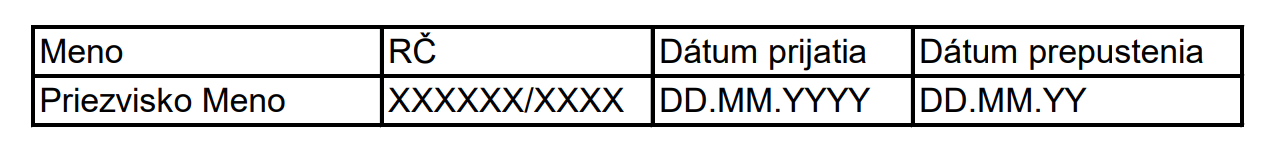
\includegraphics[width=0.9\textwidth]{images/hlavicka_a}}
	%popis obrazku
	\caption[Hlavička a)]{Výzor hlavička pacienta ktorý nebol preložený na JIS}
	%id obrazku, pomocou ktoreho sa budeme na obrazok odvolavat
	\label{obr:hlav_a}
\end{figure}

\begin{figure}
	%vlozenie samotneho obrazku vycentrovaneho a vhodnej velkosti
	%obrazok je v subore images/cervik.png
	\centerline{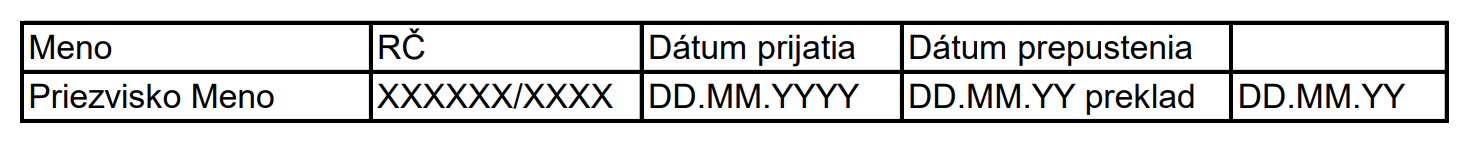
\includegraphics[width=1\textwidth]{images/hlavicka_b}}
	%popis obrazku
	\caption[Hlavička b)]{Výzor hlavička pacienta ktorý bol preložený na JIS}
	%id obrazku, pomocou ktoreho sa budeme na obrazok odvolavat
	\label{obr:hlav_b}
\end{figure}

Softvér z tejto tabuľky vyberie hodnoty z druhého riadka pričom v prípade, že v štvrtom stĺpci nájde informáciu o preklade na iné oddelenie tak dátum v tomto stĺpci ignoruje a za dátum prepustenia považuje dátum v piatom stĺpci.

Dátumy prijatia a prepustenia sú následne pre-typované do podoby časovej značky čím sa zároveň skontroluje platnosť dátumu (či taký dátum môže existovať) v prípade, že pri niektorom z dátumov vyskytne problém je táto informácia zapísaná do logovacieho súboru. V prípade, že sú obe dátumy v poriadku je následne spravený ich rozdiel čím sa vypočíta dĺžka hospitalizácie, čiže počet dní medzi prijatím a prepustením pričom tento výsledok nám dáva ďalšiu kontrolu dátumov keďže očakávame, že dĺžka hospitalizácie je kladné číslo avšak nepredpokladáme, že to číslo bude veľmi veľké, konkrétne pri testovaní sa ukázalo, že priemerná dĺžka hospitalizácie je približne 12 dní pričom štandardná odchýlka je približne 9 dní avšak občas sa objavia aj prípady ktorých dĺžka hospitalizácie je cez 50 dní pričom nenastal žiaden preklep pri zapisovaní dátumom preto sme sa rozhodli použiť ako hornú hranicu hodnotu 100 ktorá pokrývala všetky naše doterajšie prípady.

Nakoniec v prípade, že dátum prijatia je v poriadku tak softvér určí z rodného čísla dátum narodenia a pomocou dátumu narodenia a dátumu prijatia vypočíta vek pacienta pri prijatí. Tento vek následne kontroluje či je v intervale 0 až 120, v prípade, že do tohto intervalu nepatrí indikuje to chyba buď v dátume prijatia alebo v rodnom čísle pacienta.

\section{JIS a smrť}

Keďže naše dáta sú prepúšťacie správy iba z infekčného oddelenia tak nevieme čo sa s pacientom dialo po opustení oddelenia avšak to čo nás zaujíma je, že dôvod opustenia oddelenia konkrétne to čo nás zaujíma je, že či sa mu stav zhoršil na toľko, že musel byť preložený na jednotku intenzívnej starostlivosti respektíve či dôvodom na opustenie oddelenia nebolo úmrtie pacienta.

V prípade preloženia na JIS je táto informácia v časti ''Epikríza'' (\ref{blokE}) pričom je väčšinou zapísaná ako ''prekladáme na JIS'' respektíve ''prekladnáme na jednotku intenzívnej starostlivosti'' pričom avšak keďže sa táto informácia do epikrízi píše iba v prípade, že preklad uskutočnil tak sa ukázalo, že je vhodnejšie v nej hľadať iba informáciu ''JIS'' respektíve ''jednotka intenzívnej starostlivosti'' keďže pri hľadaní aj informácie ''prekladáme na'' sa vyskytlo viac prípadov keď mal systém problém túto informáciu odhaliť z dôvodu rôzneho skloňovania a gramatických chýb.

V prípade smrti pacienta sa na koniec epikrízi napíše informácia ''exitus lethalis''. Avšak ukázalo sa, že nie vždy sa táto informácia v správe nachádza aj napriek tomu, že smrť nastal čo je spôsobené tým, že smrť nastala na jednotke intenzívnej starostlivosti alebo sa na ňu z nejakého dôvodu zabudlo preto sa po komunikácii s pánom doktorom Sabakom rozhodlo, že v prípade, že bol pacient preložený na jednotku intenzívnej starostlivosti alebo bol pripojený na umelú pľúcnu ventiláciu a v správe sa nenachádza informácia o smrti tak sa táto situácia zaznamená do logovacieho súboru aby to mohol užívateľ správnosti informácie skontrolovať.

\section{Výška a váha}

Ďalšie informácie ktoré sa o pacientovi získavali boli jeho výška a váha, pričom následne bola z týchto hodnôt ešte počítaná hodnota BMI. Ukazuje sa, že existuje viacero spôsobov akými lekári zapisujú túto informáciu do správy pričom našou snahou je aby náš systém zvládal nachádzať túto informáciu pri všetkých možnostiach zápisu. Tieto spôsoby sú následovné:

\begin{itemize}
	\item {[výška/váha/hmotnosť]} {[hodnota]}{[cm/kg]} (názov a hodnota)
	\item {[hodnota]}{[cm/kg]},{[hodnota]}{[cm/kg]} (hodnoty oddelene čiarkou)
	\item {[hodnota]}{[cm/kg]}/{[hodnota]}{[cm/kg]} (hodnoty oddelene medzerou)
	\item {[hodnota]}{[cm/kg]} {[hodnota]}{[cm/kg]} (hodnoty oddelene lomkou)
\end{itemize}   

Systém kontroluje prítomnosť každej z týchto možností v texte správy a v prípade nájdenie zhody túto informáciu následne čistí rozdelením v prípade ak sa jedná o dve hodnoty oddelené nejakým deličom a následným odstránením všetkých nepodstatných informácii tak aby nakoniec ostali iba číselné informácie pričom však systém si stále pamätá ktorá hodnota prislúcha ktorej informácii (či ide o výšku alebo váhu). Následne je táto číselná hodnota kontrolovaná či je v ''rozumnom'' intervale pričom pre výšku je využívaný interval 20-250 cm a pre váhu je interval 10-300 kg ak sa nájde hodnota ktorá nepatrí do týchto intervalov je to považované za možnú chybu a informácia o tom je zapísaná do logovacieho súboru, takisto za chybu sa považuje aj prípad ak systém nedokázal nájsť niektorú z týchto informácii v texte.

V prípade nájdenia oboch informácii (aj výšky aj váhy) je z týchto hodnôt počítaná hodnota BMI pričom tak ako predchádzajúce hodnoty aj táto je kontrolovaná či sa nachádza v ''rozumnom'' intervale 10-60, vďaka tejto kontrole vieme zachytiť aj chyby s výškou a váhou ktoré nie su evidentné z jednotlivých informácii, medzi takéto prípady patria napríklad chyby ako vymenenie hodnôt výšky a váhy lekárom (príklad z textu správy ''výška/váha: 75cm/150kg'') alebo možná chyba v niektorom údajov (príklad z textu správy ''výška/váha: 103cm/90kg''), samozrejme ani v jednom prípade si nemôžeme byť istý či chyba naozaj nastala a aká konkrétne je a preto v takýchto prípadoch údaje považujeme za priebežne správne a do logovacieho súboru dávame informáciu užívateľovi aby správnosť údajov skontroloval. 

\section{Saturácia krvi kyslíkom pri prijatí}
\label{saturacia}

Jednou z ďalších informácii ktorá nás zaujímala bola saturácia krvi kyslíkom. Táto informácia bola pre nás zaujímavá keďže sa jedná o pacientom s ochorením COVID-19 ktoré sa zväčša prejavuje ako respiračné ochorenie a saturácia krvi kyslíkom je zaujímavý ukazovateľ stavu pacienta. Konkrétne nás zaujímala táto hodnota pri prijatí aby sme mali predstavu v akom stave bol pacient hospitalizovaný. 

Pri hľadaní sme postupovali tak, že sme hľadali kľučové slovo respektíve skratku (konkrétne sa jednalo o slová ''SpO2'' alebo ''SatO2'' a ich varianty) nasledované číselnou hodnotou pričom občas sa stávalo, že medzi hľadaným slovom a hodnotu sa nachádzala ešte informácia ''bez kyslíka'' označujúca, že bola meraná pred podaním oxygenoterapie pacientovi.

V prípade, že systém našiel v texte viackrát zapísanú informáciu o saturácii krvi kyslíkom tak za správnu považoval tú ktorá sa nachádza v texte najskôr keďže sa informácia pri prijatí zväčša píše do časti ''Anamnéza'' (\ref{blokB}) ktorá sa nachádza na začiatku správy.

Občas sa objavila situácia, že hodnota nebolo jedno číslo ale bol to interval (príklad z textu správy ''SatO2: 90-93\%''). V takomto prípade sme sa rozhodli považovať za skutočnú hodnotu dolnú hranicu tohto intervalu.

V prípade nenájdenia žiadnej hodnoty je informácia o tom zapísaná do logovacieho súboru. 

\section{Protilátky proti vírusu SARS-CoV-2 pri prijatí}
\label{protilatky}

Keďže náš systém analyzuje prepúšťacie správy pacientov s ochorením COVID-19 tak jednou z pre nás veľmi zaujímavých informácii je výsledok testu na protilátky proti tomuto ochoreniu. Pri hľadania výsledkov testov na protilátky sa ukázalo, že každý lekár ich zapisuje iným spôsobom pričom aj v správach jedného lekára sa nachádzajú rozdiel medzi jednotlivými zápismi. Niekoľko konkrétnych ukážok je na obrázku \ref{obr:proti}. 

\begin{figure}
	%vlozenie samotneho obrazku vycentrovaneho a vhodnej velkosti
	%obrazok je v subore images/cervik.png
	\centerline{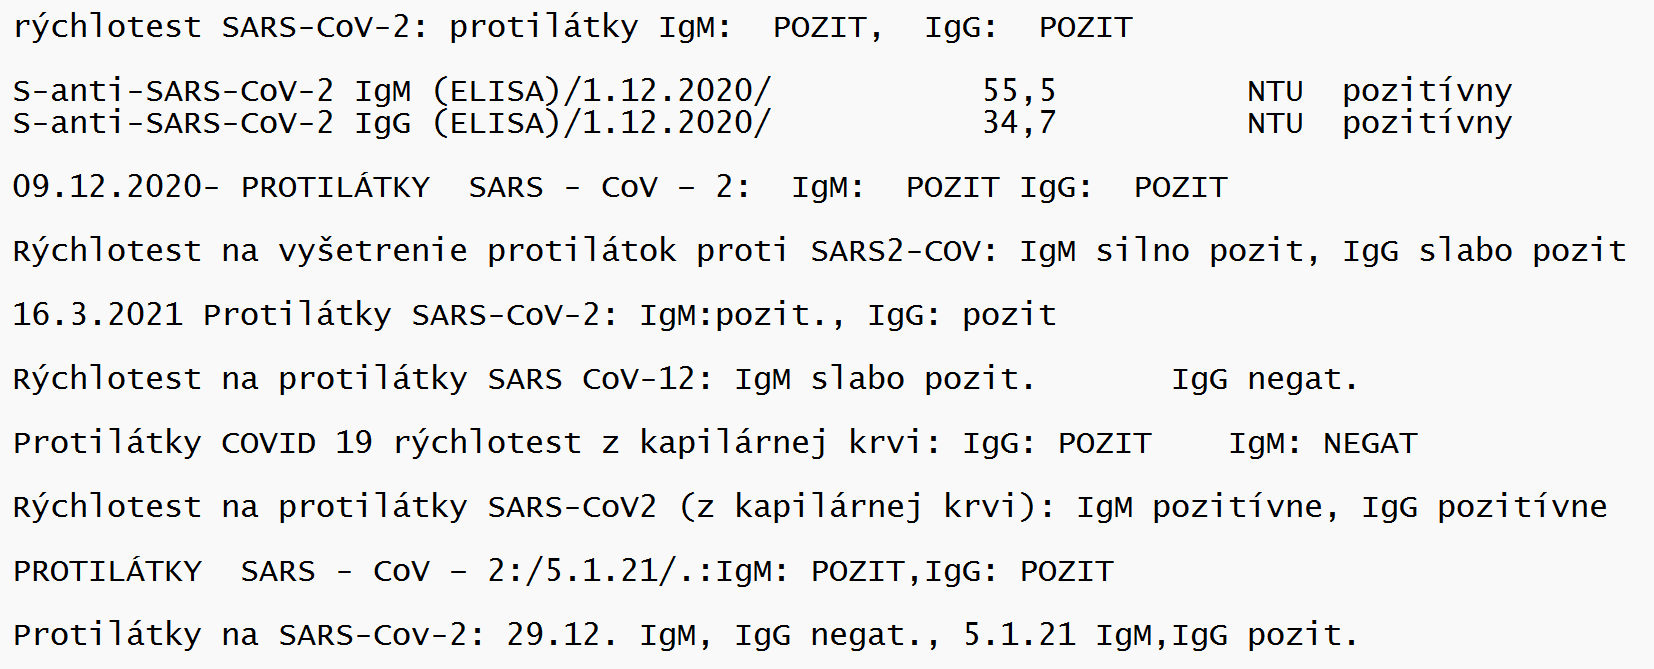
\includegraphics[width=1\textwidth]{images/protilatky}}
	%popis obrazku
	\caption[Protilátky]{Rôzne spôsoby zápisu testov na protilátky v prepúšťacích správach}
	%id obrazku, pomocou ktoreho sa budeme na obrazok odvolavat
	\label{obr:proti}
\end{figure}

Pri hľadaní a následnom získavaní informácie sme využili fakt, že všetky spôsoby zápisu týchto testov obsahujú rovnaké respektíve podobné kľúčové slová a pre nás dôležitú informáciu v rovnakom poradí konkrétne vždy prvým kľúčovým slovom je názov vírusu alebo názov choroby v našom prípade je to vírus SARS-CoV-2 respektíve v niektorých prípadoch ochorenie COVID-19, následne ide kombinácia typov protilátok, konkrétne IgG a IgM, a samotných výsledkov testov. Ukážka zvýraznenia hľadaných slov je na obrázku \ref{obr:proti_high}.

\begin{figure}
	%vlozenie samotneho obrazku vycentrovaneho a vhodnej velkosti
	%obrazok je v subore images/cervik.png
	\centerline{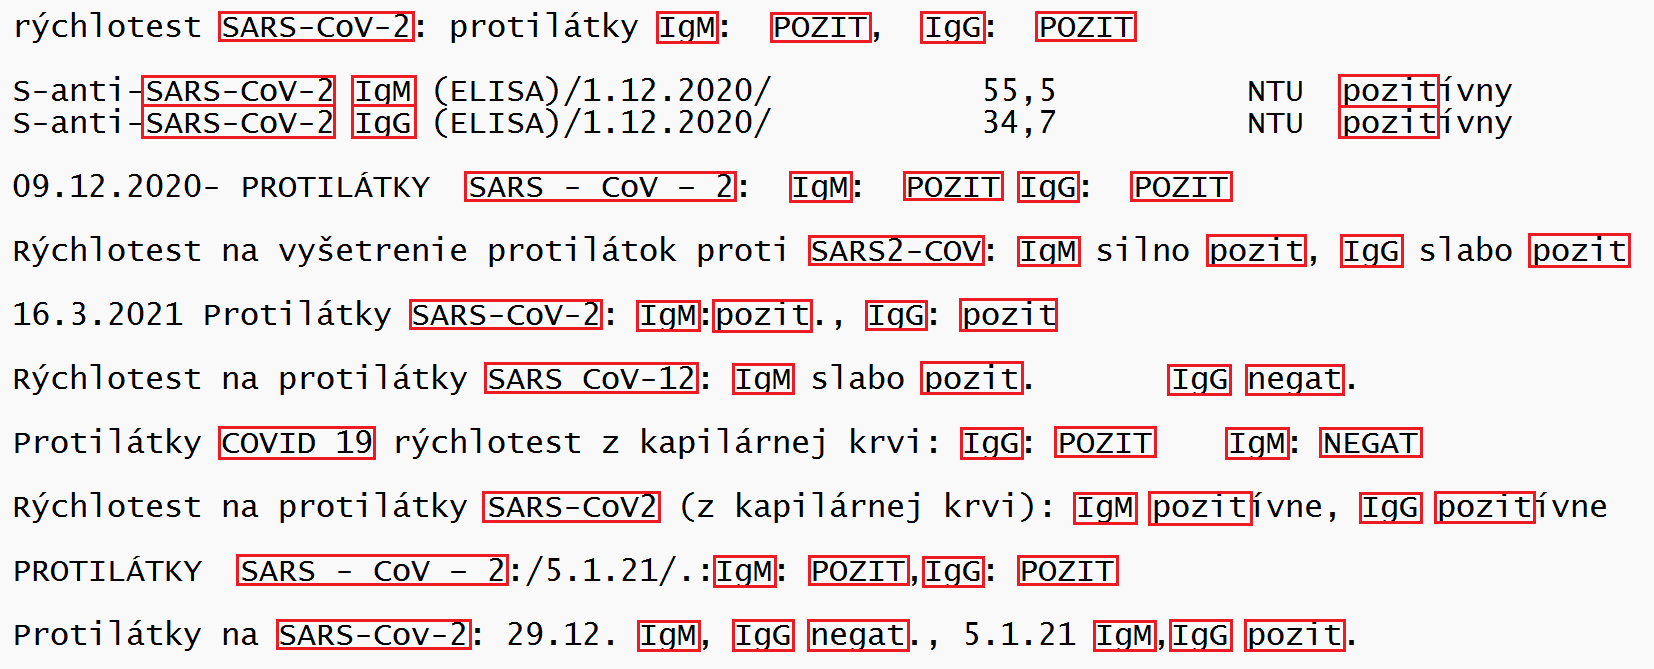
\includegraphics[width=1\textwidth]{images/protilatky_highlight}}
	%popis obrazku
	\caption[Protilátky zvýraznené]{Zvýraznené hľadaná informácie v rôznych spôsoboch zápisu testov na protilátky}
	%id obrazku, pomocou ktoreho sa budeme na obrazok odvolavat
	\label{obr:proti_high}
\end{figure}

Systém najskôr nájde celé úryvky textu obsahujúce testy následne z týchto úryvkov odstráni všetky slová a znaky ktoré sú pre samotný výsledok nepodstatné ako napríklad slová ''slabo'', ''silno'' alebo ''rýchlotest''. Keďže systém nájde iba špecificky testy na protilátky proti SARS-CoV-2 je pre nás v nájdenom úryvku nepodstatná táto informácia. Nakoniec nám ostanú iba názvy protilátok a výsledky pričom sa ukazuje, že vyskytujú v dvoch formách a to dvojice protilátka a výsledok alebo ako jeden spoločný výsledok pre obe protilátky. V testovaných prípadoch sa vždy vyskytol názov protilátky pred výsledkom testu avšak nakoniec sme sa rozhodli spraviť systém všeobecnejší tým, že prípadov keď je výsledok za názvom testu je schopný správne rozlíšiť a spracovať aj prípady keď je poradie opačné. Konkrétne v prípade nájde iba jeden 
názov protilátky (obrázok \ref{obr:proti_high} druhý príklad) a iba jeden výsledok poradie je jasne určené, v ostatných prípadoch sa rozhoduje podľa tabuľky \ref{tab:proti}.

\begin{table}[]
	\caption[Rozhodia systému pri testoch]{Rozhodnutia systém pri rôznych poradiach názvov testov a ich výsledkov}
	\label{tab:proti}
	\begin{tabular}{|p{8cm}|p{6.7cm}|}
		\hline
		\textbf{Poradie častí}                          & \textbf{Rozhodnotie}                                                                                             \\ \hline
		[protilátka] [výsledok] [protilátka] [výsledok] & názov protilátky pred výsledkom                                                                        \\ \hline
		[protilátka] [protilátka] [výsledok]            & názov protilátky pred výsledkom                                                                        \\ \hline
		[výsledok] [protilátka] [výsledok] [protilátka] & názov protilátky za výsledkom                                                                          \\ \hline
		[výsledok] [protilátka] [protilátka]            & názov protilátky za výsledkom                                                                          \\ \hline
		[protilátka] [výsledok] [protilátka]            & problém (systém považuje daný test nejasne zapísaný)          \\ \hline
		[výsledok] [protilátka] [výsledok]              & problém (systém považuje daný test nejasne zapísaný) \\ \hline
	\end{tabular}
\end{table}

V prípade, že sa v správe nachádza viacero testov na protilátky proti vírusu SARS-CoV-2 zaujíma nás ten najstarší. Pôvodne bola snaha využiť dátumy avšak ukázalo sa, že veľkom počte prípadov informácia o dátume testovania chýba preto sme sa rozhodli tento postup nevyužiť. Ďalším pokusom bola heuristická úvaha, že čím skôr je test v správe tým je starší, táto heuristika však vykazovala príliš vysokú chybovosť preto sme ani ju nevyužili. Nakoniec sme sa po debate s pánom doktorom Sabakom rozhodli využiť heuristickú úvahu, ktorá hovorí, že ak existuje test na určitú protilátky s negatívnym výsledkom tak aj najstarší test bude mať negatívny výsledok a naopak ak test s negatívnym výsledkom neexistuje (a existujú s pozitívnym výsledkom) tak aj najstarší je má pozitívny výsledok. Táto heuristika sa opiera o výsledky štúdie ktorá ukázala, že test na protilátky typu IgM je pozitívny aj po viac ako 60 dňoch od nástupu príznakov a v prípade protilátok typu IgG je to až 90 dní \cite{antibodies}. Keďže bola väčšina pacientov hospitalizovaná výrazne kratšie obdobie ako 60 dní tak nepredpokladáme, že by počas hospitalizácie nastala situácia, že pacientovi vyjde negatívny výsledok testu aj napriek pozitivite predchádzajúceho. Zároveň sa ukazuje, že ak pacientovi vyjde pozitívny test na obe protilátky už ďalší test na protilátky nie je vykonaný keďže ani lekár zväčša nepredpokladá, že by množstvo protilátok v krvi počas hospitalizácie výrazne kleslo.

\section{Oxygenoterapia}

V prípade oxygenoterapie sme zo správy získavali dve informácie a to či bola pacientovi podaná oxygenoterapia a ak bola určiť o aký typ oxygenoterapie išlo. Konkrétne rozlišujeme tri základné typy a low-flow, HFNO (high-flow nasal oxygenotherapy) a UPV (umelú pľúcnu ventiláciu). 

V prípade, že systém nenašiel žiadnu informáciu (žiadne kľučové slová) o podaní oxygenoterapie zapísal si k pacientovi informáciu ''bez oxygenoterapie'' v opačnom prípade sa typ určí na základe toho aké kľúčové slová boli v texte nájdené. Konkrétne systém nájdené slová vyhodnocuje následovne:

\begin{itemize}
	\item ''low flow'', ''low-flow'' a podobne - low-flow
	\item ''high flow'', high-flow'', ''HFNO'' a podobne - HFNO
	\item ''umelá pľúcna ventilácia'', ''UPV'' a podobne - UPV
\end{itemize}

V prípade, ak sa v texte nachádza informácie aj o low-flow aj o HFNO alebo UPV tak je informácia o low-flow zanedbaná keďže ide o menej ''extrémny'' typ. Avšak v prípad ak sa v správe nachádza informácia aj o HFNO aj o UPV sú do výslednej informácie o pacientovi zapísané obe a to v tvare ''HFNO/UPV''. Ak v správe nebol typ oxygenoterapie presne určený ale nachádzala sa tam iba informácie o spôsobe podania ako "maska" alebo "nosová kanyla" je to považované za low-flow oxygenoterapiu pričom do výslednej informácie o pacientovi je to zapísané ako ''low-flow (neupresnené)'' aby bolo jasne označené, že konkrétna informácii o typu nie je v správe prítomná.

\section{Lieky}

Získavanie informácie sa ukázalo ako veľmi priamočiare keďže našou snahou nebolo získať množinu liekov ktorú pacient dostával ale mali sme množinu liekov a zisťovali sme ktoré z nich pacient dostával. Dôvodom pre tento prístup bol fakt, že pacienti často dostávali lieky a vitamíny určené na liečby iných problémov ktorými títo pacienti trpeli a pre nás bola dôležitá len množina liekov ktoré mohli byť použité na liečbu ochorenia COVID-19. Konkrétne išlo o tieto lieky: Dexametazon, Remdesivir, Olumiant, Favipiravir, Ivermectin a Colchicin.

Konkrétne hľadanie týchto liekov bolo zisťovanie či sa názov lieku nachádza v správe, zo začiatku sme skúšali hľadanie iba v časti ''Terapia'' (\ref{blokD}) avšak nakoniec sme sa rozhodli hľadať v celej správe aby sme predišli prípadom keď v správe je informácia o danej liečbe ale táto informácia sa už nedostala do terapie a takisto sme chceli zachytiť prípady kedy išlo o samoliečbu pacienta respektíve lieky predpísané obvodným lekárom ktoré už ale po hospitalizácii neužíval (hlavne v prípade lieku Ivermectin). Keďže sa nenašli prípady kedy by lekár do správy zapísal informáciu o lieku ktorý pacient neužíval tak sa tento spôsob hľadania informácie o týchto liekoch ukázal ako najspoľahlivejší.
 
Boli aj snahy zistiť okrem samotných liekov aj informáciu o počte dní počas ktorých boli tieto lieky pacient užíval a dávku lieku ktorá mu bola predpísaná avšak sa ukázalo, že vo výraznej väčšine správ buď táto informácia úplne chýba alebo je neúplná a tieto informácie z nej nie je možné získať preto nakoniec padlo rozhodnutie nezískavať tieto informácie.

\section{Choroby pacienta}

Keďže pri ochorení COVID-19 tak ako aj pri iných ochoreniach sa niektoré iné diagnózy považujú za rizikové faktory. Preto aj našou snahou bolo sa pokúsiť získať informáciu či pacient niektorou z diagnóz považovaných za možné rizikové faktory trpí respektíve ju prekonal. Našťastie pre nás sa táto informácia často nachádza v časti ''Anamnéza'' (\ref{blokB}) avšak môže sa objaviť aj iných častiach správy keďže k danému problému môže dôjsť aj počas hospitalizácie.

Konkrétne diagnózy ktorých prítomnosť alebo prekonanie u pacienta sa snažíme určiť sú následovné: cukrovka, artériová hypertenzia, srdcové zlyhanie, infarkt myokardu, fibrilácia predsiení, periférne artériové ochorenie dolných končatín, chronická obštrukčná choroba pľúc, astma, cievna mozgová príhoda, demencia, sepsa a kolitída. Pričom v prípade ochorení sepsa a kolitída nás nezaujíma či ich pacient v minulosti prekonal ale či sa vyskytli pri prijatí alebo počas hospitalizácie.

V prípade väčšiny týchto chorôb je ich získavanie priamočiare, konkrétne sa jedná o zisťovanie či sa v texte správy nachádza informácia o tejto chorobe u pacienta či už vo forme celého názvu (pri niektorých chorobách niektorého z viacerých používaných názvov napríklad cukrovka a diabetes alebo periférne artériové ochorenie dolných končatín a ateroskleróza) alebo vo forme skratky (napríklad CHOCHP pre chronická obštrukčná choroba pľúc alebo IM pre infarkt myokardu). Tento postup sa ukázal ako vhodný aj pre sepsu keďže prekonanie tejto choroby sa nezapisuje do anamnézy a v anamnéze respektíve v správe sa vyskytuje iba v prípade ak ňou pacient trpí pri alebo počas hospitalizácie.

Špecifické bolo určovanie kolitídy pri alebo počas hospitalizácie. V tomto prípade sa ukázal problém, že veľmi často informácia, že sa v správe nachádza názov tohto ochorenia neznamená automaticky prítomnosť tohto ochorenia u pacienta ale môže isť o negatívny výsledok testu na toto ochorenie alebo prípad, že toto ochorenia bolo pacientom prekonané v minulosti. Konkrétny prístup ktorý sme sa rozhodli použiť pre čo najlepšie určenia prítomnosti tohto ochorenia u pacienta je tvorený dvomi časťami. Najskôr prebehne kontrola či sa v správe nachádza hocijaká informácie o tomto ochorení čiže či sa tam nachádza názov (kolitída alebo clostridium difficile) alebo skratka (CDI) tejto choroby, v prípade ak sa v správe nenachádza žiadna informácia tak to systém považuje za prípad keď pacient na kolitídu počas hospitalizácie netrpel. Ak sa nejaká informácia o tomto ochorení v správe nachádza nasleduje druhá časť hľadanie kedy hľadáme informáciu o teste na toto ochorenie, konkrétny spôsob hľadania a vyhodnocovania testov na toto ochorenie je podobný ako zisťovanie výsledkov testov na protilátky proti vírusu SARS-CoV-2 (\ref{protilatky}) s rozdielom, že namiesto SARS-CoV-2 hľadáme clostridium difficile a keďže ide o test na prítomnosť protilátok ale baktérie nás netrápi typ (pri SARS-CoV-2 sme rozlišovali IgG a IgM protilátky). V prípade ak sa nájde pozitívny test tak tvrdíme, že pacient počas hospitalizácie na toto ochorenie trpel, naopak v prípade, že všetky nájdené testy sú negatívne tak tvrdíme, že pacient netrpel na toto ochorenie počas hospitalizácie, špeciálny prípad je ak systém nenájde žiaden test na toto ochorenie v takom prípade systém nevie určiť správny výsledok a preto zapíše informáciu o tomto probléme do logovacieho súboru aby to mohol užívateľ skontrolovať.

\section{Krvné výsledky}

Záverečná ale najväčšia skupina informácii ktoré sme získavali boli niektoré výsledky krvných testov. Nie su pre nás dôležité všetky výsledky ale iba určitá vybraná podmnožina konkrétne ide o výsledky ktoré sa v laboratórnych výsledkov označujú nasledujúcimi skratkami: CRP, PCT, S\_D3, GLU, KREA, ALT, GMT, FERR, TnT, NEU\#, LYM\#, EO\#, PLT, CD4A, CD8A, INR, FBG, DD. 

Hľadanie týchto výsledkov by sa dalo rozdeliť na dve časti a to hlavné hľadanie a doplnkové hľadanie. V prípade hlavného hľadania sú tieto údaje hľadané časti správy ''Krvné výsledky'' (\ref{blokG}). Konkrétne hľadá informácie v tvare ''[názov]: [hodnota]'' pričom následne z toho získame samotnú číselnú hodnotu. Priebežne si zapamätáva aj informáciu ktoré údaje nenašiel, v tomto prípade chýbajúci údaj nie je nutne chybou keďže nie každému pacientovi boli robené rovnako komplexné krvné testy. Po pokuse o získania všetkých údajov nastáva druhá časť ktorou je doplnkové hľadanie v tejto časti sa údaje ktoré sa nepodarilo nájsť v časti ''Krvné výsledky'' hľadajú v texte samotnej prepúšťacej správy. Hlavným dôvodom pre toto hľadanie boli prípady kedy či už z nejakého dôvodu sme nedostali úplné krvné výsledky alebo bolo počas hospitalizácie robených viacero nezávislých krvných testov pričom my sme dostali iba niektoré ale výsledky týchto testov boli zapísané do správy. Tieto dáta sa nachádzajú v správe v časti ''Vyšetrenia'' (\ref{blokC}) avšak ako bolo aj pri popise výzoru vstupných dát vysvetlené v tejto časti sa často nachádza iba nejaký výber výsledkov ktorý nemusí obsahovať tie ktoré my potrebujeme. Problém ktorý sa objavuje v tejto časti je fakt, že pre určitý údaj sa v správe môže nachádzať viacero hodnôt keďže ten istý test bol počas hospitalizácie spravený pacientovi niekoľkokrát v takom prípade je informácia zapísaná v tvare ''[názov]: [hodnota 1]; [hodnota 2]; ... [hodnota n],'' pričom v takom prípade my berieme prvú hodnotu keďže tieto hodnoty sú usporiadané v poradí v akom boli testy robené (časovo) a nás zaujíma hodnota najbližšie k začiatku hospitalizácie keďže chceme vedieť v akom stave bol pacient na začiatku nemocničnej liečby.

V prípade, že ani hlavné, ani doplnkové hľadanie nenájde nejaké výsledky testov je informácie o ich nenájdený zapísaná do logovacieho súboru avšak keďže táto informácia sa nemusí nutne v správe nachádzať nie je táto informácia zapísaná medzi chyby ktoré sa pri získavaní informácii objavili ale je samostatne označená ako nenájdené výsledky testov. V prípade, že sa pri doplnkovom hľadaní zistí, že sa výsledok testu objavuje v správe viackrát pričom sú pri ňom odlišné hodnoty je to považované za chybu a informácia o tejto chybe je zapísaná do logovacieho súboru.

\section{Chýbajúce časti vstupu}

Vo väčšine prípadov je výzor našich presne taký ako je popísaný v kapitole ''Štruktúra prepúšťacej správy'' (\ref{kap:strukSpravy}) avšak občas sa objavil problém neúplnosti dát. Konkrétne išlo o prípady kedy sa vo vstupnom texte nenachádzali výsledky krvných testov, v takom prípade jediná zmena ktorú systém spraví je, že pri získavaní údajov z krvných výsledkoch preskočí hlavné hľadanie (keďže nemá na to potrebný text) a údaje získava iba pomocou doplnkového hľadania v texte prepúšťacej správy. Občas sa objavili ešte extrémnejší prípad kedy sme pre dané pacienta dostali iba hlavička (\ref{blokA})  a informácia ''chýba správa'' v takomto prípade sa zo získavania dát vykoná iba získavanie osobných údajov pacient a obdobia jeho hospitalizácie (\ref{osobUdaj}) aby bola zachovaná existencia tohto pacienta a logovacieho súboru sa zapisuje informácia o chýbajúcej správe.

\section{Výstupné súbory}   

Výsledkom celého získavania informácie zo vstupných dát je dvojica súborov, ide o súbor vo formáte XLSX ktorý je možné otvoriť v programe Microsoft Excel a obsahuje tabuľku v ktorej jednotlivé riadky sú pacienti a stĺpce sú jednotlivé získavané údaje, druhým súborom je textový logovací súbor obsahujúci pre každého spracovávaného pacienta v tvare zobrazenom na obrázku \ref{obr:log}.

\begin{figure}
	%vlozenie samotneho obrazku vycentrovaneho a vhodnej velkosti
	%obrazok je v subore images/cervik.png
	\centerline{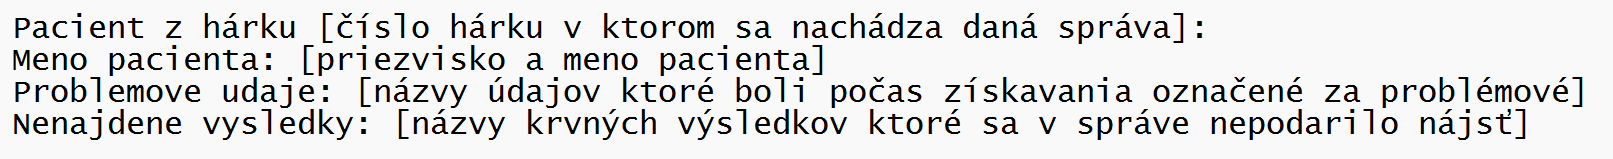
\includegraphics[width=1\textwidth]{images/log_subor}}
	%popis obrazku
	\caption[Logovací súbor]{Výzor zápisu informácie o chýbajúcich a problémových údajoch v logovacom súbore pre jedného pacienta}
	%id obrazku, pomocou ktoreho sa budeme na obrazok odvolavat
	\label{obr:log}
\end{figure}    
